
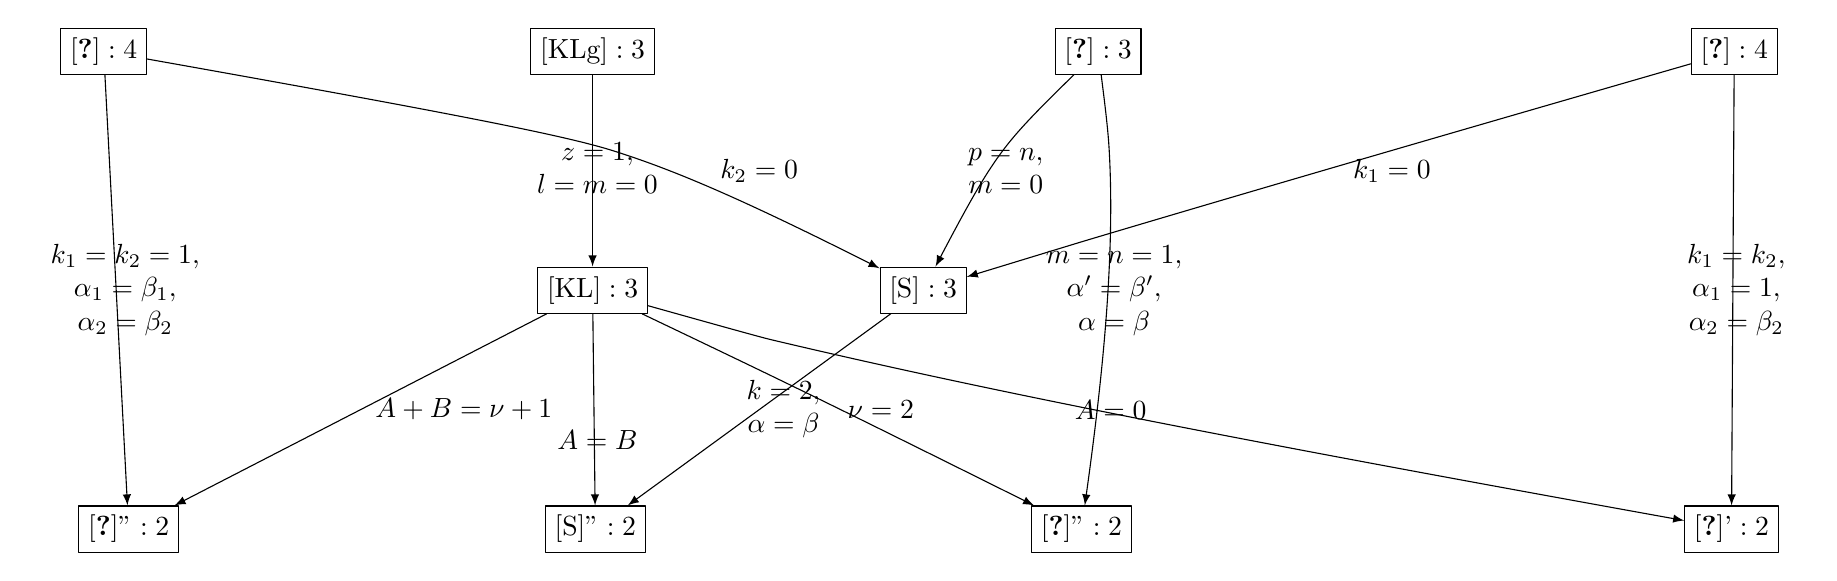
\begin{tikzpicture}[>=latex,line join=bevel,]
%%
\begin{scope}
  \pgfsetstrokecolor{black}
  \definecolor{strokecol}{rgb}{1.0,1.0,1.0};
  \pgfsetstrokecolor{strokecol}
  \definecolor{fillcol}{rgb}{1.0,1.0,1.0};
  \pgfsetfillcolor{fillcol}
\end{scope}
\begin{scope}
  \pgfsetstrokecolor{black}
  \definecolor{strokecol}{rgb}{1.0,1.0,1.0};
  \pgfsetstrokecolor{strokecol}
  \definecolor{fillcol}{rgb}{1.0,1.0,1.0};
  \pgfsetfillcolor{fillcol}
\end{scope}
\begin{scope}
  \pgfsetstrokecolor{black}
  \definecolor{strokecol}{rgb}{1.0,1.0,1.0};
  \pgfsetstrokecolor{strokecol}
  \definecolor{fillcol}{rgb}{1.0,1.0,1.0};
  \pgfsetfillcolor{fillcol}
\end{scope}
  \node (DF85) at (455.64bp,190.0bp) [draw,rectangle] {$\mbox{\cite{dotsenko1985four}}:3$};
  \node (Spp) at (274.64bp,18.0bp) [draw,rectangle] {$\mbox{[S]''}:2$};
  \node (KL) at (273.64bp,104.0bp) [draw,rectangle] {${\mbox{[KL]}}:3$};
  \node (S) at (392.64bp,104.0bp) [draw,rectangle] {$\mbox{[S]}:3$};
  \node (KLg) at (273.64bp,190.0bp) [draw,rectangle] {${\mbox{[KLg]}}:3$};
  \node (War10) at (97.64bp,190.0bp) [draw,rectangle] {$\mbox{\cite{warnaar2010sl3}}:4$};
  \node (War10pp) at (106.64bp,18.0bp) [draw,rectangle] {$\mbox{\cite{warnaar2010sl3}''}:2$};
  \node (DF85pp) at (449.64bp,18.0bp) [draw,rectangle] {$\mbox{\cite{dotsenko1985four}''}:2$};
  \node (TV03) at (684.64bp,190.0bp) [draw,rectangle] {$\mbox{\cite{tarasov2003selberg}}:4$};
  \node (TV03p) at (683.64bp,18.0bp) [draw,rectangle] {$\mbox{\cite{tarasov2003selberg}'}:2$};
  \draw [->] (KLg) ..controls (273.64bp,160.36bp) and (273.64bp,145.43bp)  .. (KL);
  \definecolor{strokecol}{rgb}{0.0,0.0,0.0};
  \pgfsetstrokecolor{strokecol}
  \draw (275.39bp,147.0bp) node {$\begin{array}[]{c}z=1,\\l=m=0\end{array}$};
  \draw [->] (DF85) ..controls (458.71bp,166.05bp) and (459.32bp,159.78bp)  .. (459.64bp,154.0bp) .. controls (461.71bp,116.65bp) and (457.41bp,73.587bp)  .. (DF85pp);
  \draw (461.39bp,104.0bp) node {$\begin{array}[]{c}m=n=1,\\ \alpha'=\beta',\\\alpha=\beta\end{array}$};
  \draw [->] (TV03) ..controls (574.86bp,158.3bp) and (509.18bp,139.17bp)  .. (451.64bp,122.0bp) .. controls (450.2bp,121.57bp) and (448.73bp,121.13bp)  .. (S);
  \draw (561.39bp,147.0bp) node {$k_1=0$};
  \draw [->] (KL) ..controls (323.37bp,80.247bp) and (336.57bp,73.886bp)  .. (348.64bp,68.0bp) .. controls (366.74bp,59.174bp) and (386.62bp,49.362bp)  .. (DF85pp);
  \draw (377.39bp,61.0bp) node {$\nu=2$};
  \draw [->] (TV03) ..controls (684.36bp,141.98bp) and (684.01bp,81.897bp)  .. (TV03p);
  \draw (685.39bp,104.0bp) node {$\begin{array}[]{c}k_1=k_2,\\ \alpha_1=1,\\\alpha_2=\beta_2\end{array}$};
  \draw [->] (KL) ..controls (333.11bp,87.331bp) and (335.9bp,86.647bp)  .. (338.64bp,86.0bp) .. controls (416.07bp,67.675bp) and (504.09bp,50.383bp)  .. (TV03p);
  \draw (481.39bp,61.0bp) node {$\kern-1.5cm A=0$};
  \draw [->] (War10) ..controls (100.15bp,141.98bp) and (103.3bp,81.897bp)  .. (War10pp);
  \draw (105.39bp,104.0bp) node {$\begin{array}[]{c}k_1=k_2=1,\\\alpha_1=\beta_1,\\\alpha_2=\beta_2\end{array}$};
  \draw [->] (DF85) ..controls (431.2bp,166.27bp) and (425.7bp,160.11bp)  .. (421.14bp,154.0bp) .. controls (415.87bp,146.94bp) and (410.85bp,138.81bp)  .. (S);
  \draw (422.39bp,147.0bp) node {$\begin{array}[]{c}p=n,\\m=0\end{array}$};
  \draw [->] (KL) ..controls (273.98bp,74.36bp) and (274.16bp,59.434bp)  .. (Spp);
  \draw (275.39bp,61.0bp) node {$\begin{array}[]{c}\\\\A=B\end{array}$};
  \draw [->] (S) ..controls (350.36bp,73.186bp) and (326.63bp,55.893bp)  .. (Spp);
  \draw (342.39bp,61.0bp) node {$\begin{array}[]{c}k=2,\\\alpha=\beta\end{array}$};
  \draw [->] (War10) ..controls (230.5bp,166.37bp) and (265.12bp,159.26bp)  .. (281.64bp,154.0bp) .. controls (304.42bp,146.75bp) and (328.73bp,136.15bp)  .. (S);
  \draw (333.59bp,147.0bp) node {$k_2=0$};
  \draw [->] (KL) ..controls (213.02bp,72.785bp) and (178.11bp,54.803bp)  .. (War10pp);
  \draw (202.39bp,61.0bp) node {$\kern5emA+B=\nu+1$};
%
\end{tikzpicture}
